\documentclass[10pt,twocolumn]{article}

\usepackage[a4paper,top=16mm,bottom=18mm,left=15mm,right=15mm,columnsep=6mm]{geometry}
\usepackage{fontspec}
\setmainfont{TeX Gyre Termes}
\setsansfont{TeX Gyre Heros}
\setmonofont{DejaVu Sans Mono}[Scale=0.82]
\usepackage{microtype}
\usepackage{graphicx}
\graphicspath{{../figures/}}
\usepackage{booktabs}
\usepackage{array}
\usepackage{amsmath,amssymb}
\usepackage{siunitx}
\usepackage[font=small,labelfont=bf]{caption}
\usepackage{xcolor}
\usepackage{enumitem}
\usepackage[numbers,sort&compress]{natbib}
\usepackage[colorlinks=true,allcolors=blue!55!black]{hyperref}

\definecolor{auditblue}{HTML}{0072B2}
\definecolor{auditamber}{HTML}{E69F00}
\definecolor{auditred}{HTML}{D55E00}
\newcommand{\jtext}{J-TEXT}
\newcommand{\east}{EAST}
\newcommand{\tpr}{\mathrm{TPR}}
\newcommand{\fpr}{\mathrm{FPR}}
\newcommand{\method}{\textsc{Causal-Private Active Transfer}}
\newcommand{\devstatus}{\textsc{Test-Driven Exploration}}
\sisetup{detect-all,round-mode=places,round-precision=3}
\setlength{\parindent}{1em}
\setlength{\parskip}{0pt}
\setlist{nosep,leftmargin=*}

\title{Audit-first cross-tokamak disruption prediction with feature-semantic transfer and causal active adaptation}
\author{Anonymous authors\\[-1mm]\small Development manuscript---not an independent deployment claim}
\date{}

\begin{document}
\maketitle

\begin{abstract}
Cross-tokamak disruption prediction is a small-target-data problem complicated by diagnostic mismatch, unequal discharge duration, and non-stationary campaigns.  We develop an audit-first three-stage pipeline from \jtext{} to \east{}: a causal patch Transformer trained on 17 physically reconstructible features; target adaptation using a fixed 110-shot \east{} support roster whose HDF5-authoritative labels are 15 disruptive and 95 non-disruptive; and chronological active adaptation that supplements the shared representation with eight \east{}-private channels.  Every online shot follows \emph{predict--seal--query--reveal--update}, so a current outcome can affect only later shots.  Across seeds 131/133/137, the same primary lineage obtains on a non-chronological, count-aligned \jtext{} TEST220 comparator a mean operational TPR at lead $>10$ ms of 0.852, FPR of 0.212, AUC of 0.922, and lead-qualified median of 116.6 ms.  After few-shot transfer, static evaluation on a chronological balanced360 \east{} development stream gives a mean operational TPR at lead $\geq30$ ms of 0.841, FPR of 0.167, and lead-qualified median of 242.0 ms.  Online adaptation changes these to 0.848, 0.152, and 229.5 ms.  A strict support110 EAST-only baseline gives TPR 0.796, FPR 0.144 and median lead 165.6 ms; transfer improves TPR$_{30}$--FPR by 0.022 and lead by 76.5 ms while increasing FPR by 0.022.  On query-label-disjoint complements, front-loading the same queried shots into ordinary target refitting raises TPR at 30 ms by 0.064 but raises FPR by 0.167, reducing TPR$_{30}$--FPR by 0.103 in all three seeds; the causal online path exceeds this front-loaded control by 0.116.  In a causal block-matched random-query replay, the full active mechanism exceeds the within-seed random mean by 0.016, but it realizes 2.21 times more inter-shot update attempts.  A separate fixed-operator control gives every queried shot exactly 16 current and 16 support windows plus two shared and two private optimizer attempts; archived-active minus random-mean TPR$_{30}$--FPR is then $-0.00185$, 0, and $-0.00556$.  Thus archived-roster superiority is unsupported under this operator; the adaptive selector-policy effect is not estimated.  A paired circular moving-block resample (block 20) gives a descriptive online-minus-static FPR change of $-0.0139$ (95\% interval $[-0.0352,-0.0019]$), but the same stream informed architecture and 972-candidate parameter development, so none of these analyses is confirmatory inference.  Moreover, a same-endpoint padding audit rejects the primary source representation; removing that shortcut reduces source sensitivity and causes negative transfer under the frozen online policy.  The study therefore supplies a reproducible coupled mechanism and falsification analysis, not independent generalization or deployment evidence.
\end{abstract}

\noindent\fcolorbox{auditamber}{auditamber!10}{\parbox{0.96\columnwidth}{\small\textbf{Evidence status.} All \east{} balanced360 numbers are \devstatus{}.  The \jtext{} validation/test roles are outcome-balanced, count-aligned comparators rather than strict chronological blocks.  The 360-shot stream was used to develop the architecture and parameter range; no demonstrably pristine local future stream remains.  Neither stage is an independent deployment confirmation.}}

\section{Introduction}

Disruption prediction must identify a hazardous plasma evolution early enough to support mitigation while avoiding unnecessary interventions.  Transferring a model between tokamaks is attractive because target-device disruptive shots are scarce, yet naively aligning raw channels can confound diagnostic calibration, machine geometry, campaign state, class prevalence, and evolution time scale.  The original parameter-based \jtext{}$\rightarrow$\east{} study addressed this problem with device-specific physics-guided feature extraction and target-side fine-tuning, and reported that lower local representations transfer more readily than upper temporal representations~\citep{zheng2023transfer,shen2023pgfeda}.  Its thesis protocol further used a 110-shot target support set and a balanced 360-shot target evaluation roster~\citep{shen2024thesis}.  These observations motivate transfer through physical semantics, but they do not by themselves guarantee causal online operation or eliminate shortcut learning.

Domain alignment is not automatically beneficial.  CORAL aligns second-order statistics~\citep{sun2016coral}; domain-adversarial training attempts to erase domain information~\citep{ganin2016dann}.  Both can fail when label conditionals or support differ, and domain-adaptation impossibility results formalize why unlabeled marginal alignment alone cannot identify the correct target predictor~\citep{bendavid2010impossibility}.  In this project, direct alignment of the nominal 23 dimensions repeatedly produced negative transfer.  Inspection showed that several columns were not physically or numerically comparable between devices.  A second failure mode arose from source-window padding: discharge length and relative temporal context were predictive enough to become shortcuts, a general failure pattern in deep models~\citep{geirhos2020shortcut}.

We therefore ask a narrower question: \emph{with the labels and diagnostics already available, what can be supported about a low-cost, causal \jtext{}$\rightarrow$\east{} transfer-and-adaptation chain?}  Our contributions are:

\begin{enumerate}
  \item a label-authoritative and feature-semantic data contract that distinguishes a 17-dimensional cross-device subspace from eight \east{}-private observations;
  \item an end-to-end causal active protocol in which unlabeled intra-shot updates, label queries, outcome reveals, and inter-shot updates have explicit information boundaries;
  \item a same-lineage, three-seed development evaluation with per-shot ledgers, hashes, moving-block resampling, chronological blocks, shortcut probes, negative controls, and alarm-parameter robustness;
  \item a same-label-access counterfactual that separates the availability of queried labels from their delayed, guarded online use; and
  \item a failure-preserving ablation: PADFIX removes the measurable source padding shortcut, but its reduced sensitivity and incompatibility with the frozen target policy expose a genuine robustness--transfer trade-off rather than a hidden success.
\end{enumerate}

\section{Data and causal contract}

\subsection{Authoritative cohorts}

The local HDF5 stores contain 1,733 \jtext{} shots (378 disruptive/1,355 non-disruptive) and 2,953 \east{} shots (1,198/1,755).  For every reported outcome, \texttt{/meta/IsDisrupt} and \texttt{/meta/DownTime} are the sole label authority; text shot lists are roster provenance only.  The executed \jtext{} roles are TRAIN1353 (188/1,165), VAL160 (80/80), and TEST220 (110/110), with zero shot overlap and individually hashed rosters.  They are a fixed paper131-count-aligned cohort: each roster is sorted for serialization, but the role ranges overlap in shot number and \emph{do not} form strict chronological blocks.  Source parameters and scaling are fitted on TRAIN1353; epoch and alarm threshold are selected on the balanced VAL160; TEST220 is held out within this execution.  Because its membership is outcome-balanced and it does not mimic source prevalence or prospective chronology, TEST220 is a within-run comparator, not independent deployment evidence.

The \east{} transfer roster contains 110 shots and has no overlap with balanced360.  Its legacy list headings say 10 disruptive/100 non-disruptive, but HDF5 truth is \textbf{15/95}; the latter is used throughout.  All 110 shots are used for target fitting and the support-derived operating threshold, so there is no separate target validation cohort and only 15 disruptive support outcomes.  The chronological balanced360 stream contains 180/180 and is sorted by shot identifier.  Figure~\ref{fig:protocol} summarizes the contract.  Because balanced360 informed method development, we use it only for diagnostic comparisons.  We do not retrofit an ``unseen'' label to it.

\begin{figure*}[t]
  \centering
  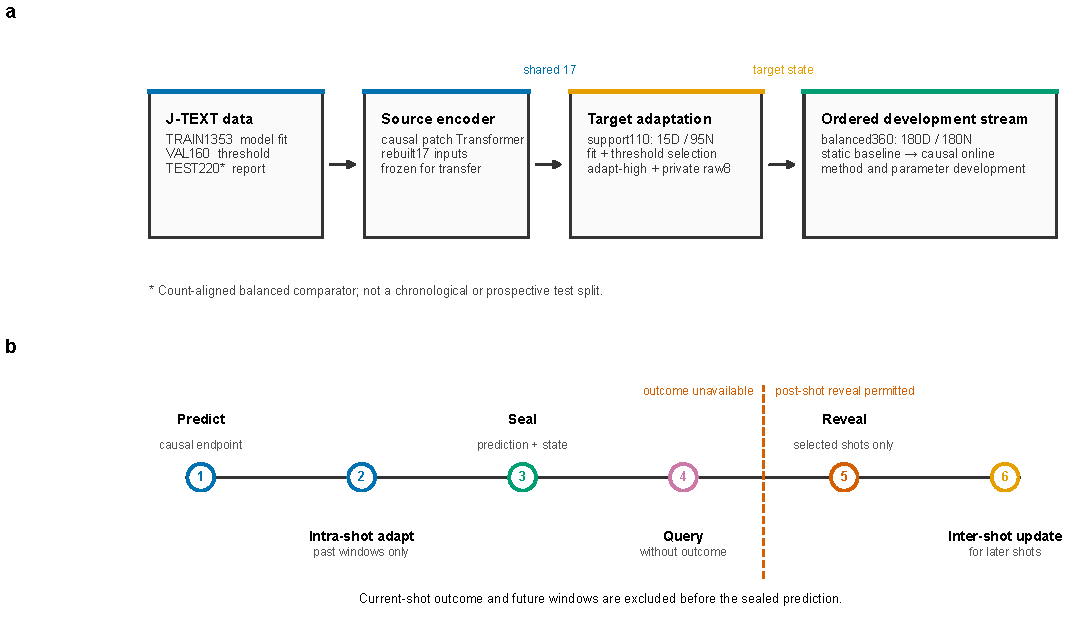
\includegraphics[width=\textwidth]{fig1_protocol_and_causal_contract.pdf}
  \caption{Three-stage data flow and causal online protocol.  The roster labels are recomputed from HDF5; the 110-shot transfer and 360-shot development rosters are disjoint.  The current-shot outcome is inaccessible until prediction, alarm, and query decision are sealed.}
  \label{fig:protocol}
\end{figure*}

\subsection{Cross-device and private features}

The nominal raw vector has 23 columns.  We reconstruct a 17-dimensional shared vector with single-conversion plasma current in amperes, toroidal field, $B_t/I_p$, $\Delta I_p$, loop voltage, $V_{\rm loop}/I_p$ as a causal impedance proxy, soft-X-ray and extreme-ultraviolet distribution statistics, available MHD frequency/amplitude summaries, mode number, and position proxies.  Missingness is represented by an availability mask and unavailable values are set to zero only after robust scaling.

Eight columns are excluded from cross-device alignment because their units, availability, or diagnostic realization are not reliably comparable: CIII, MNM, Mirnov vertical/amplitude summaries, $n_e/n_G$, $q_a$ proxy, SXR mean, and XUV ratio.  They are not discarded.  A target-private sidecar computes six causal summaries per channel (last value, mean, standard deviation, full-window increment, recent increment, and availability fraction), uses a 16-unit two-layer SiLU network, starts from a zero residual, and bounds its logit correction.  Its robust median/IQR scaler is fitted only on the 110 \east{} support shots.  This separation follows the physics-guided principle of mapping device-specific diagnostics to common semantics~\citep{zheng2023transfer,shen2023pgfeda}, while avoiding the unsupported assumption that every raw column is cross-device invariant.

\section{Model and adaptation}

\begin{figure*}[t]
  \centering
  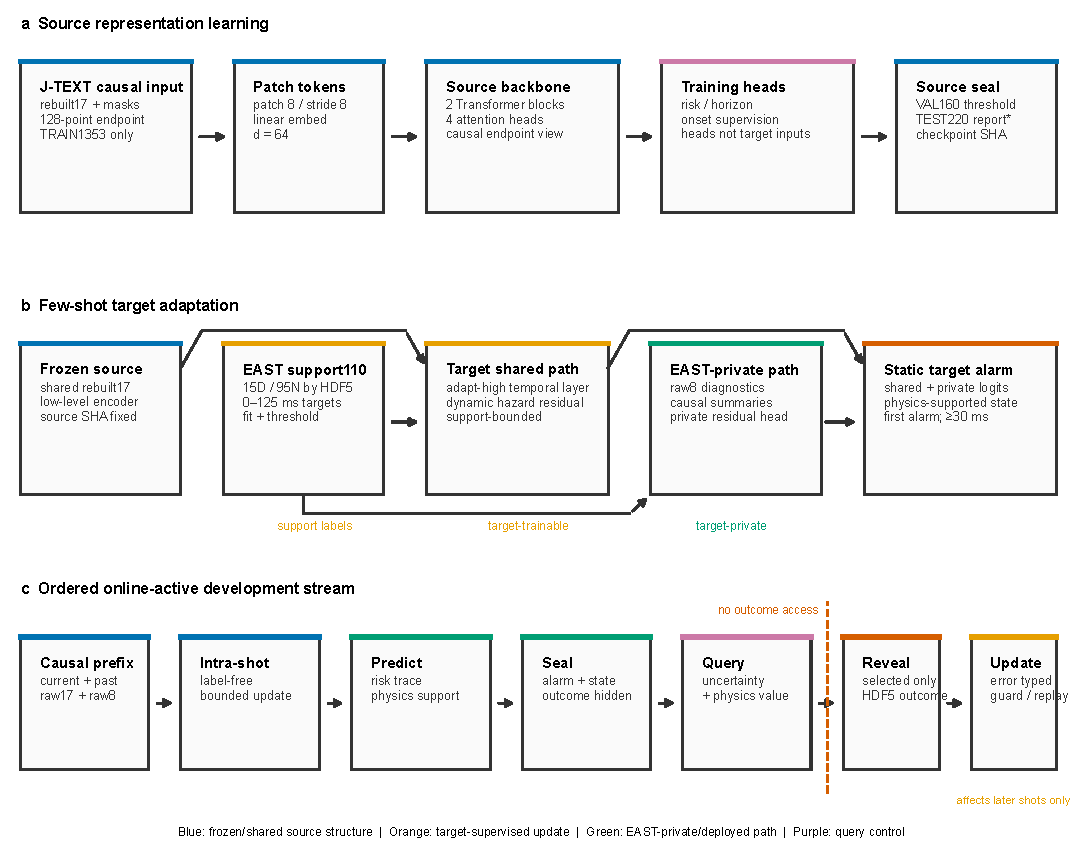
\includegraphics[width=\textwidth]{fig0_end_to_end_model_architecture.pdf}
  \caption{Executed model and adaptation architecture.  \textbf{a}, A causal 17-feature \jtext{} endpoint is patch-embedded and encoded by the source Transformer; onset and horizon signals supervise training heads but are not target-time inputs.  \textbf{b}, support110 adapts the target shared temporal/risk path and fits a separate eight-diagnostic \east{}-private residual before the fixed static alarm is evaluated.  \textbf{c}, each ordered online shot permits bounded label-free intra-shot adaptation before prediction and sealing; only queried outcomes cross the dashed information boundary, and any guarded supervised update can affect later shots only.  Colours identify computational roles rather than evidence strength.}
  \label{fig:architecture}
\end{figure*}

\subsection{Source model}

Figure~\ref{fig:architecture} separates the source, target-supervised and online-update paths.  For a causal endpoint $t$, the source input is a 128-sample history of 17 features.  A convolutional patch embedding with patch and stride 8 yields 16 temporal tokens.  A learned class token, sinusoidal positions, two pre-normalized Transformer layers (model width 64, four heads, feed-forward width 256), and a two-layer risk head produce logit $z_{s,t}$.  This is the actual executed architecture, \texttt{128x8-d64-l2-h4}; earlier planning documents mentioning a 256-sample window are not used by this lineage.  Patch Transformers provide the architectural template~\citep{nie2023patchtst}.

Windows are sampled evenly by class and by shot.  A disruptive endpoint is positive when its time to disruption (TTD) lies in $[0,125]$ ms; earlier endpoints and all safe endpoints are negative under the registered sampling rules.  The binary cross-entropy objective is
\begin{equation}
\mathcal{L}_{\rm src} = -y\log\sigma(z)-(1-y)\log(1-\sigma(z)).
\end{equation}
The VAL160 operating point is the highest threshold attaining operational $\tpr_{>10\,\mathrm{ms}}\geq0.90$ with minimum FPR.  A single supported threshold crossing is the registered alarm; consecutive-ten-point results are not substituted for it.

\subsection{Few-shot target transfer}

The shared source representation initializes the target path.  The effective transfer design adapts target temporal/risk components on support110 rather than globally forcing the two marginal distributions to coincide.  It then adds: (i) a small target dynamic-hazard path that reads frozen class, terminal, and lagged latent changes together with available physics-family summaries; and (ii) the target-private raw-eight residual.  Target positive supervision uses the \east{} 125-ms hazard horizon.  The same support110 selects the target threshold at a nominal support TPR of 0.8; this is target development, not an unbiased validation estimate.  Source checkpoints and the shared parent are hash-checked before and after target adaptation; deployment uses an independent target risk path rather than the source risk score as a privileged input.

The alarm is a causal two-route state machine.  It combines normalized risk margin $m_t$, causal physics support $p_t$, and a fast--slow trend:
\begin{equation}
\begin{aligned}
E_t &= m_t+w_{p,t}p_t
+w_{r,t}[\operatorname{MA}_{5}(m)_t-\operatorname{MA}_{100}(m)_t]_+,\\
\mathcal A_t&=\mathbf{1}\{m_t\ge h_t\}\lor\mathbf{1}\{E_t\ge e_t\}.
\end{aligned}
\label{eq:alarm}
\end{equation}
Here $h_t,w_{p,t},w_{r,t},e_t$ are the adaptive high threshold, physics weight, trend weight, and early threshold; moving-average widths 5/100 are fixed.  A disruptive shot is an operational TP only when its first accepted alarm precedes HDF5 DownTime by at least 30 ms; an alarm below 30 ms is an operational FN.  Alarms earlier than 3 s remain eligible under this rule but are separately audited because they may reflect campaign/shot state rather than a useful precursor.

\subsection{Two-time-scale online adaptation}

Test-time adaptation can update normalization or model parameters without labels~\citep{wang2021tent,niu2022eata,wang2022cotta}; active continual adaptation additionally allocates labels under a budget~\citep{zhou2022online}.  Our protocol separates four values that must not be conflated:

\begin{enumerate}
  \item \emph{intra-shot value}: next-state reconstruction error, teacher disagreement, physics contradiction, raw-eight innovation, availability, non-redundancy, and alarm proximity scale a resettable fast update using current and past windows only;
  \item \emph{query value}: uncertainty and physics contradiction select labels with a past-only block-frozen threshold; a five-expert decision value is logged in shadow mode after direct control degraded performance;
  \item \emph{post-reveal update value}: the sealed prediction error determines FP/FN/TARDY/TP/TN-specific residual, replay, and projected alarm updates; and
  \item \emph{deployment veto value}: a 60-dimensional causal alarm-episode representation estimates false-alarm probability from previously queried outcomes and may only delay or veto a supported alarm.
\end{enumerate}

The state transition is
\begin{equation}
\theta_{s}^{-}\xrightarrow[\text{unlabelled}]{x_{s,\leq t}}\tilde\theta_{s,t}
\xrightarrow{\text{seal}}(\hat y_s,q_s)
\xrightarrow[\text{selected only}]{y_s}\theta_{s+1}^{-}.
\end{equation}
Fast state is reset at the next shot; persistent target residuals and alarm parameters are protected by support replay and rollback.  The source encoder and source head remain frozen.  Crucially, the deployment veto is isolated from the counterfactual learning alarm: correcting an FP cannot relabel that same shot as a TN inside the learning trajectory and thereby alter later updates.

After a queried label is revealed, FP feedback makes the two-route alarm stricter, FN/TARDY feedback advances it and strengthens early evidence, and TP/TN trajectories become protected guards.  The immutable ledgers record 38, 30, and 40 actual parameter-changing updates for seeds 131, 133, and 137, respectively.  Starting from $(h,w_p,w_r,e)=(0,8,12,7.9)$, the final tuples are
\begin{equation}
\begin{aligned}
131 &: (-0.02138,8.03083,12.01541,7.86988),\\
133 &: (-0.02180,8.07657,12.03828,7.83735),\\
137 &: (-0.01883,8.03904,12.01952,7.86219).
\end{aligned}
\end{equation}
These values demonstrate online state evolution; they are not post-hoc static threshold choices.

The selected episode rule is recalibrated from past queried data.  It requires class support and separation, uses a disruptive-class negative-score quantile plus a protection margin, fails open when separation is absent, and permits a physics-support escape.  Before freezing this rule, 972 candidates were screened on balanced360 and 55 passed the strict three-seed gate.  We preserve this multiplicity in the evidence record and do not interpret the final configuration as preregistered confirmation.

\subsection{Same-label-access front-load counterfactual}

To test whether online improvement is explained merely by obtaining more target labels, we construct a deliberately non-deployable hindsight control.  For each seed, the exact shots selected by that seed's executed query ledger are added to support110 before ordinary target refitting.  Those queried shots are then removed from scoring; static, front-loaded, and causal-online predictions are compared only on the same query-label-disjoint complement.  A support-only refit must first reproduce the archived parent encoder/head hashes, adapter hashes, support threshold, and static predictions exactly.  The original fixed support110 threshold is primary; support110 recalibration is secondary.  Three label-agnostic random front-load rosters per seed match the number of queries inside every 20-shot block.  Random replicates are averaged within seed before seeds are averaged.  This design matches label access, not historical optimizer windows, steps, FLOPs, or random-number states, which were not fully archived.

\section{Evaluation}

For each seed, the primary source, transferred static, and online models belong to the same checkpoint lineage.  The formal sensitivity is lead-qualified operational TPR: $>10$ ms for \jtext{} and $\geq30$ ms for \east{}.  Median lead is computed over those operational TPs only.  The \jtext{} per-shot ledger stores the first crossing endpoint and alarm time; its lead is recomputed from the HDF5 disruption time rather than trusted as a precomputed scalar.  We additionally report FPR, AUC where a continuous shot score is available, counts beyond 3 s, four chronological 90-shot blocks, and score correlations with shot identifier and duration.  The online phase starts from the same transferred parent as the static phase, after the entire static stream has been closed and hashed.

We use 5,000 paired circular moving-block resamples of the observed ordered ledger, with block size 20 as the displayed analysis and sizes 10, 20, 30, and 45 as sensitivity checks.  Each resample applies identical indices to all seeds and to static and online phases, preserving local order and pairing without treating three seeds as 1,080 independent shots.  The resample does not rerun the adaptive learner under a new history, and all intervals are unadjusted after 972-candidate selection on this same stream.  They are therefore descriptive stability summaries, not confidence intervals for a prospectively selected policy.  The earlier iid class-stratified bootstrap and post-hoc exact tests remain secondary diagnostics only.

\section{Results}

\subsection{Same-lineage three-stage performance}

Table~\ref{tab:primary} gives the requested three stages.  The source stage is evaluated on the count-aligned \jtext{} TEST220 comparator using a balanced-VAL160 threshold and a strict $>10$-ms minimum lead.  Target stages use the same balanced360 development roster and a $\geq30$-ms minimum lead.  All three static seeds record operational TPR above 0.82 on that reused development stream.  Online adaptation reduces FP counts from 28/26/36 to 24/24/34 and raises the total number of operational TPs by four.  The observed mean operational TPR changes by $+0.0074$ and mean FPR by $-0.0148$.

\begin{table*}[t]
\centering
\caption{Primary same-lineage operational metrics.  A \jtext{} TP requires lead $>10$ ms and an \east{} TP requires lead $\geq30$ ms.  Median lead is over lead-qualified TPs only.  A single causal supported crossing is sufficient; the mean rows are arithmetic summaries, not confidence bounds.}
\label{tab:primary}
\scriptsize
\begin{tabular}{llrrrrrrr}
\toprule
Stage & Seed & TP/FN & Operational TPR & FP/TN & FPR & AUC & Lead (ms) & Queries \\
\midrule
J-TEXT source & 131 & 97/13 & 0.8818 & 25/85 & 0.2273 & 0.9307 & 107.2 & -- \\
J-TEXT source & 133 & 90/20 & 0.8182 & 21/89 & 0.1909 & 0.9253 & 120.7 & -- \\
J-TEXT source & 137 & 94/16 & 0.8545 & 24/86 & 0.2182 & 0.9098 & 122.1 & -- \\
J-TEXT source & \textbf{mean} & -- & \textbf{0.8515} & -- & \textbf{0.2121} & \textbf{0.9219} & \textbf{116.6} & -- \\
\midrule
EAST static & 131 & 148/32 & 0.8222 & 28/152 & 0.1556 & -- & 263.0 & 0 \\
EAST static & 133 & 151/29 & 0.8389 & 26/154 & 0.1444 & -- & 205.1 & 0 \\
EAST static & 137 & 155/25 & 0.8611 & 36/144 & 0.2000 & -- & 258.0 & 0 \\
EAST static & \textbf{mean} & -- & \textbf{0.8407} & -- & \textbf{0.1667} & \textbf{--} & \textbf{242.0} & 0 \\
\midrule
EAST online & 131 & 152/28 & 0.8444 & 24/156 & 0.1333 & -- & 228.5 & 102 \\
EAST online & 133 & 151/29 & 0.8389 & 24/156 & 0.1333 & -- & 214.0 & 90 \\
EAST online & 137 & 155/25 & 0.8611 & 34/146 & 0.1889 & -- & 246.0 & 99 \\
EAST online & \textbf{mean} & -- & \textbf{0.8481} & -- & \textbf{0.1519} & \textbf{--} & \textbf{229.5} & 97.0 \\
\bottomrule
\end{tabular}

\end{table*}

For the block-20 analysis, the descriptive interval for online FPR is $[0.0897,0.2241]$ and for online operational TPR is $[0.8046,0.8877]$.  Online-minus-static intervals are $[-0.0352,-0.0019]$ for FPR, $[0.0017,0.0150]$ for operational TPR, and $[-69.01,4.00]$ ms for operational median lead.  Block sizes 10/20/30/45 retain the recorded TPR/FPR direction, but this does not constitute a significance claim: the policy was selected on the same stream and the learner was not rerun inside each resample.  No block analysis supports a stable improvement in lead time.

\begin{figure*}[t]
  \centering
  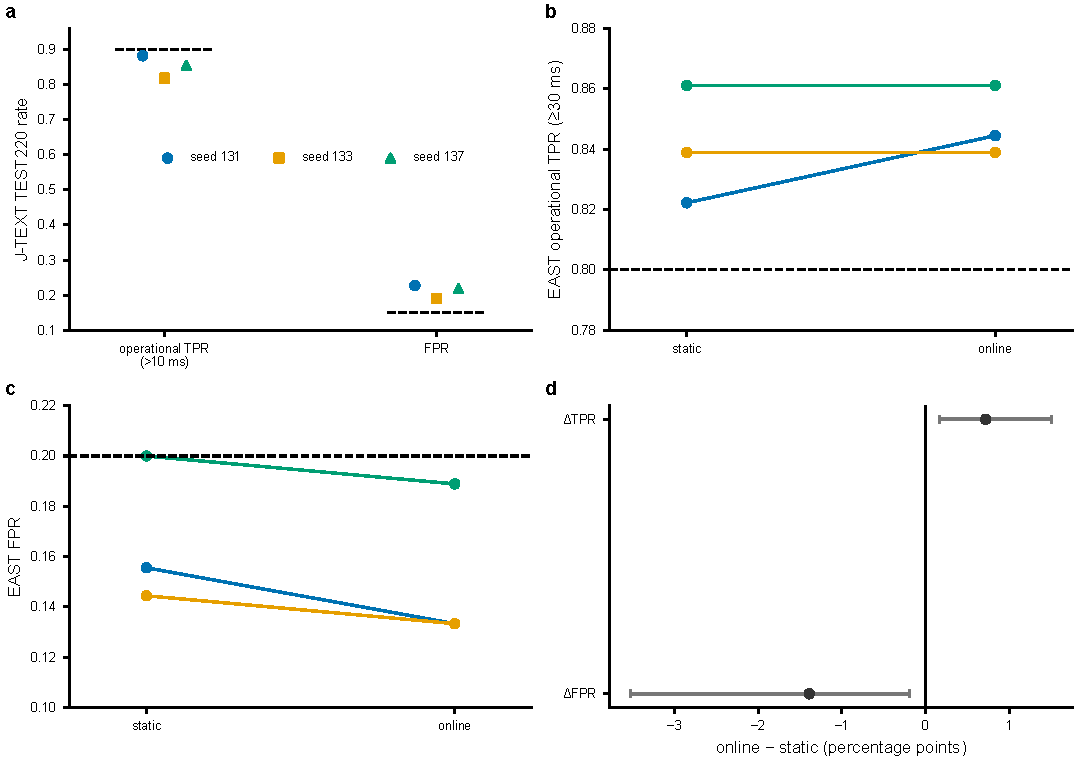
\includegraphics[width=\textwidth]{fig2_same_lineage_metrics_and_block_resampling.pdf}
  \caption{Same-lineage source and target results without implying cross-device metric continuity. (a) Per-seed \jtext{} TEST220 operational TPR and FPR; the short dashed segments mark their distinct registered gates. Source rates are not connected to target rates because the cohorts and minimum-lead rules differ. (b,c) Paired \east{} static-to-online operational TPR and FPR on the same ordered balanced360 shots. (d) Paired circular moving-block (block size 20) descriptive intervals for online-minus-static rate changes, in percentage points. The corresponding lead-time change is $-11.7$ ms with interval $[-69.0,4.0]$ ms. These intervals are post-selection stability summaries, not prospective confidence intervals.}
  \label{fig:metrics}
\end{figure*}

\subsection{Target-only controls bound the transfer contribution}

A strict \east{}-only control uses the same support110 labels, temporal window contract, 17-channel Transformer architecture, target-side shared/private modules, support-derived threshold rule and dual alarm, but initializes the entire encoder and risk head randomly and fits its scaler only on support110.  Its equal-seed means are operational TPR 0.7963, FPR 0.1444, TPR$_{30}$--FPR 0.6519 and median lead 165.6 ms.  Transfer-static changes these by $+0.0444$, $+0.0222$, $+0.0222$ and $+76.5$ ms, respectively.  Thus source transfer improves sensitivity, warning time and the combined operating objective relative to the strongest pure-target baseline, while also increasing false alarms.  The strict target-only arm itself approaches the aggregate gate but seed 133 has TPR 0.7722, so target supervision alone does not pass the declared all-seed rule.

A second random-initialization diagnostic reuses only the immutable \jtext{} scaler.  It obtains TPR 0.7315 and FPR 0.1056, demonstrating that source normalization without source weights is not a competitive \east{} baseline.  This isolates a substantive normalization mismatch but does not estimate a pure representation effect: target-only updates the full encoder whereas transfer-static updates a restricted target path, so matched optimizer steps are not equal FLOPs or equal trainable capacity.  All values remain test-driven balanced360 development evidence.

\begin{figure*}[t]
  \centering
  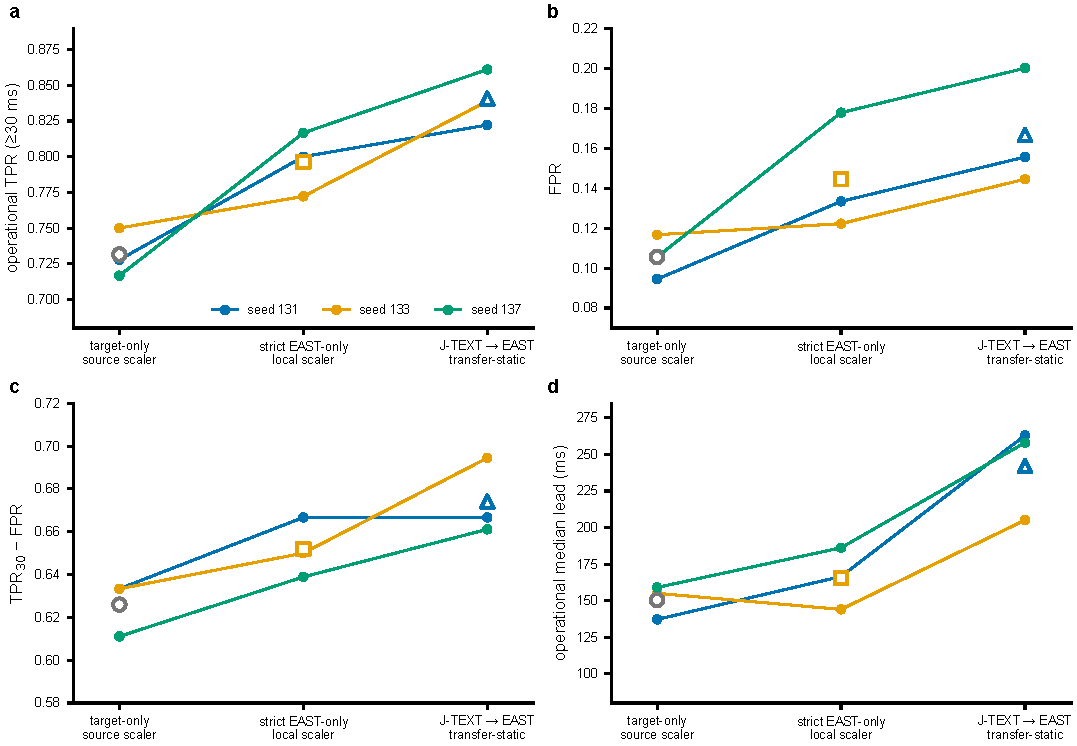
\includegraphics[width=\textwidth]{fig10_target_only_vs_transfer.pdf}
  \caption{Target-only controls and transferred static model.  Lines pair the same model seeds across a random-initialized target model with a source scaler, a strict \east{}-only model with a support-local scaler, and the transferred \jtext{} model.  Open symbols show equal-seed means.  The strict target-only control is the relevant baseline; the source-scaler diagnostic exposes normalization mismatch.  Training uses the same target window and configured optimizer-step budget but not equal trainable capacity or FLOPs.}
  \label{fig:targetonly}
\end{figure*}

\subsection{The source shortcut is real, and its repair is not free}

The primary source lineage fails a same-endpoint context audit.  For each eligible validation endpoint we retain the endpoint and supervision anchor while truncating only earlier history to 32, 64, 96, or 128 samples.  A multinomial linear probe fitted on TRAIN1353 representations predicts context bucket on VAL160 with macro-AUC 0.955/0.929/0.937, exceeding the registered maximum 0.65.  Mean absolute risk differences are 0.061/0.064/0.071 and alarm flip rates 5.7/8.6/7.0\%, also violating the 0.05 gates.  Hence the successful target lineage cannot be described as a shortcut-free mechanistic representation.

PADFIX trains on paired legal contexts, adding logit and representation consistency plus an outcome-conditional padding-bucket adversary.  With the configuration locked on VAL160, probe AUC falls to 0.624/0.645/0.649, mean risk difference to 0.011/0.009/0.008, and flip rate to 1.5/2.6/2.2\%.  However, on the once-opened TEST220, mean operational TPR falls to 0.827 while FPR improves to 0.152.  Reusing the frozen target/online policy yields static FPR 0.163 and online FPR 0.170: online adaptation increases false positives in every seed.  Figure~\ref{fig:shortcut} exposes this trade-off.  We therefore retain PADFIX as an ablation and reject it as a drop-in replacement; adapting policy geometry to a repaired parent requires a new, independently selected target study.

\begin{figure*}[t]
  \centering
  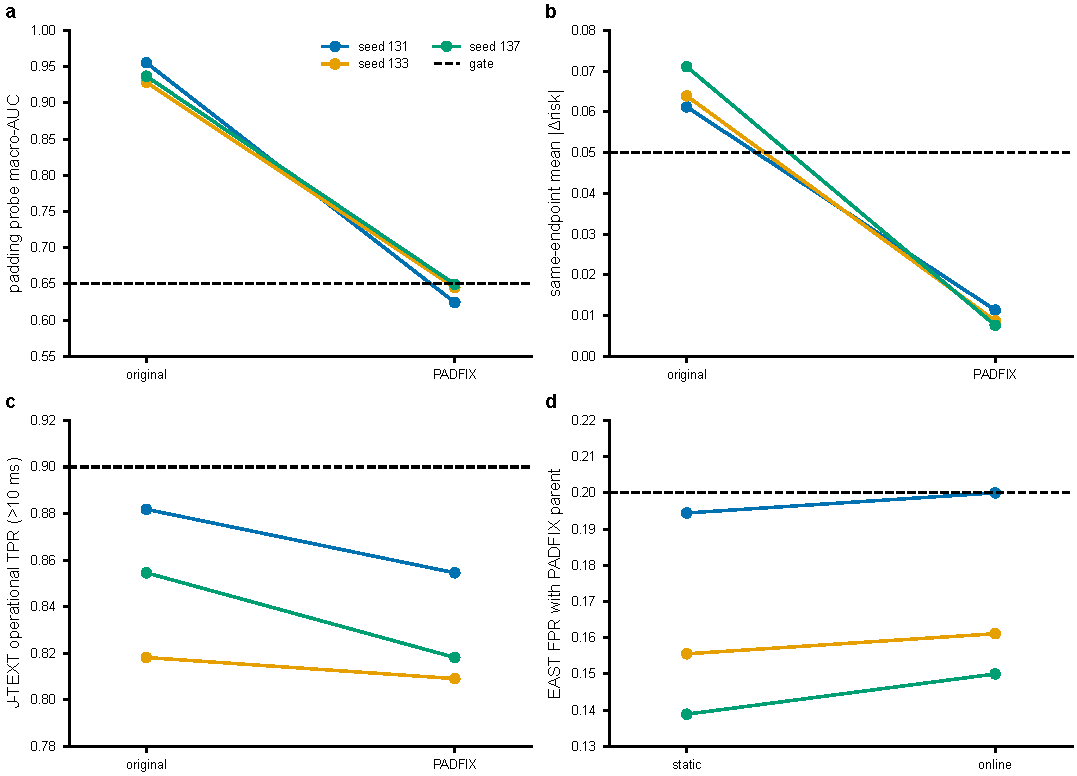
\includegraphics[width=\textwidth]{fig3_source_shortcut_and_padfix_tradeoff.pdf}
  \caption{Padding/context shortcut audit and repair. PADFIX passes all registered context gates on VAL160, but loses operational source sensitivity. The result prevents a mechanistic overclaim and demonstrates why representation repair and target-policy reuse must be evaluated jointly.}
  \label{fig:shortcut}
\end{figure*}

\subsection{Temporal drift and active-query value}

Aggregate means conceal campaign-local failure.  In four chronological blocks, online FPR reaches 0.273, 0.333, and 0.364 in block 2 for seeds 131/133/137.  Worst-block operational TPR is 0.667/0.791/0.733.  Safe-shot score correlates with shot identifier at $\rho=0.220$ for seed 131 and $\rho=0.311$ for seed 137 (the latter $p<10^{-4}$), while duration correlations are smaller.  These findings are compatible with residual campaign state and preclude a temporal-block admission claim.

Queried shots are retrospectively enriched for operational errors.  The selected-label fractions are 28.3\%, 25.0\%, and 27.5\%; operational error rates among queried shots are 0.343, 0.322, and 0.414, compared with 0.144, 0.147, and 0.164 overall.  Error enrichment is therefore 2.38, 2.19, and 2.53.  A causal random-query replay matches each active ledger's per-block label counts with three random schedules per seed.  Active TPR$_{30}$--FPR exceeds the random mean by 0.0204, 0.0093 and 0.0185 for seeds 131, 133 and 137.  However, active selection triggers 2.21 times as many realized inter-shot update attempts, the selector was developed on this stream, and three same-direction seeds give an exact one-sided sign probability of 0.125.  The result is therefore a development comparison, not prospective or equal-FLOP proof.

To remove the realized-update-attempt mediator, we replayed the archived active identities and three random rosters per seed through a separate fixed-shape assimilation operator.  Every query receives 16 current windows, 16 immutable support windows, two shared attempts and two private attempts; all intra-shot, alarm, episode and memory learners are frozen.  Active-minus-random-mean TPR$_{30}$--FPR is $-0.00185$, 0 and $-0.00556$, so the post-development reporting screen fails.  This negative screen does not establish equivalence or estimate the adaptive selector policy: it uses three random schedules on the same development stream and treats archived identities rather than rerunning that policy prospectively.  Guard decisions make committed parameter updates differ even though windows, batch shapes, scopes and optimizer attempts are matched.

\begin{figure*}[t]
  \centering
  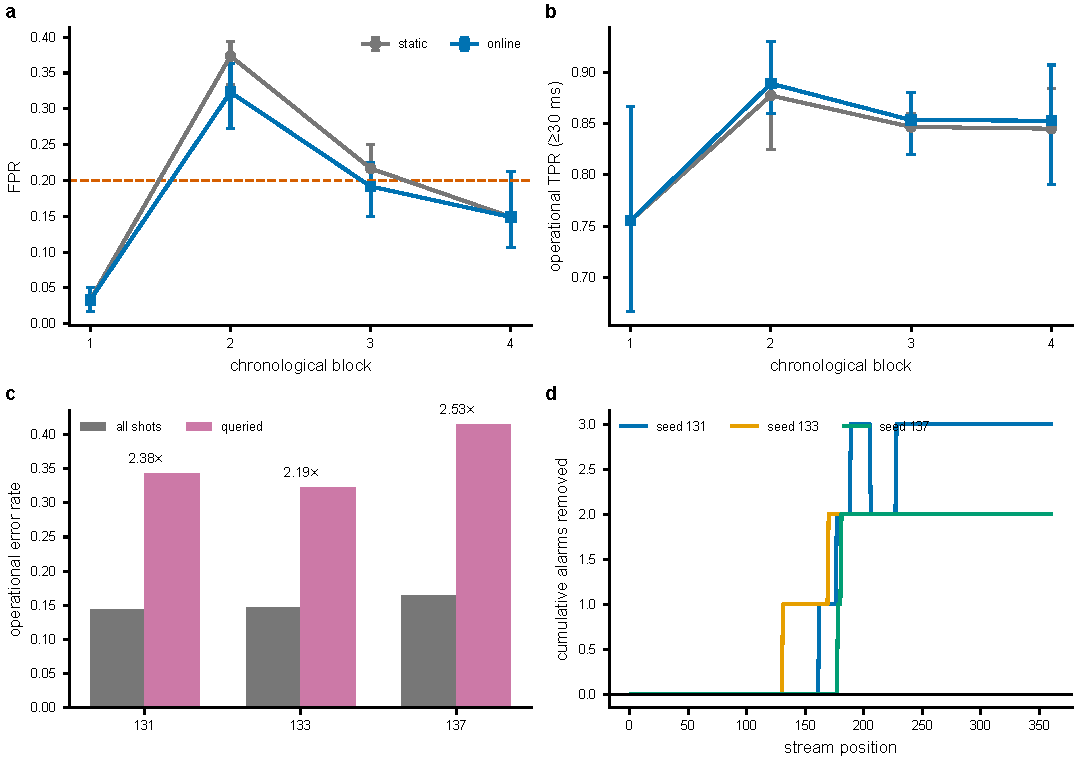
\includegraphics[width=\textwidth]{fig4_chronological_blocks_and_active_query_value.pdf}
  \caption{Chronological heterogeneity and active-query diagnostics. In (a,b), points are three-seed means and whiskers span the seedwise minimum and maximum within each fixed 90-shot block; they are not confidence intervals. Aggregate improvements coexist with a high-FPR second block. In (c), queried shots are retrospectively enriched for operational errors; this is not an equal-budget random-query comparison. Panel (d) shows the cumulative static-minus-online alarm count in stream order.}
  \label{fig:chronology}
\end{figure*}

\subsection{More labels alone do not reproduce the online gain}

The same-label-access counterfactual uses 102, 90, and 99 queried shots for seeds 131, 133, and 137; their HDF5 class counts are 61/41, 49/41, and 43/56 disruptive/non-disruptive.  The corresponding label-disjoint evaluation complements contain 258, 270, and 261 shots.  Three-seed equal-weight means on these complements are: static TPR$_{30}=0.8883$, FPR $=0.0524$, and TPR$_{30}$--FPR $=0.8359$; selected-query front-loading gives 0.9525, 0.2197, and 0.7327; causal online gives 0.8939, 0.0449, and 0.8490.  Thus front-loading raises TPR$_{30}$ by 0.0641 but FPR by 0.1673, reducing the combined operating objective by 0.1032 in every seed.  Online exceeds front-loading by 0.1163 on that objective in every seed.  Recalibrating the front-loaded model on support110 reduces the objective further to 0.7252.

The block-count-matched random front-load control shows the same sensitivity--specificity displacement.  After random replicates are averaged within seed, static, selected front-load, random front-load, and online yield TPR$_{30}$--FPR values 0.8387, 0.7322, 0.7033, and 0.8510 on their common masks.  Hence the queried labels are informative, but ordinary batch refitting shifts the global decision surface toward disruptive predictions.  The result rules out ``label count alone'' as a sufficient explanation for the observed online operating point.  The unequal-attempt random-query replay supports the full coupled treatment only descriptively; the fixed-shape screen does not support archived-roster superiority under its separate operator.

\begin{figure*}[t]
  \centering
  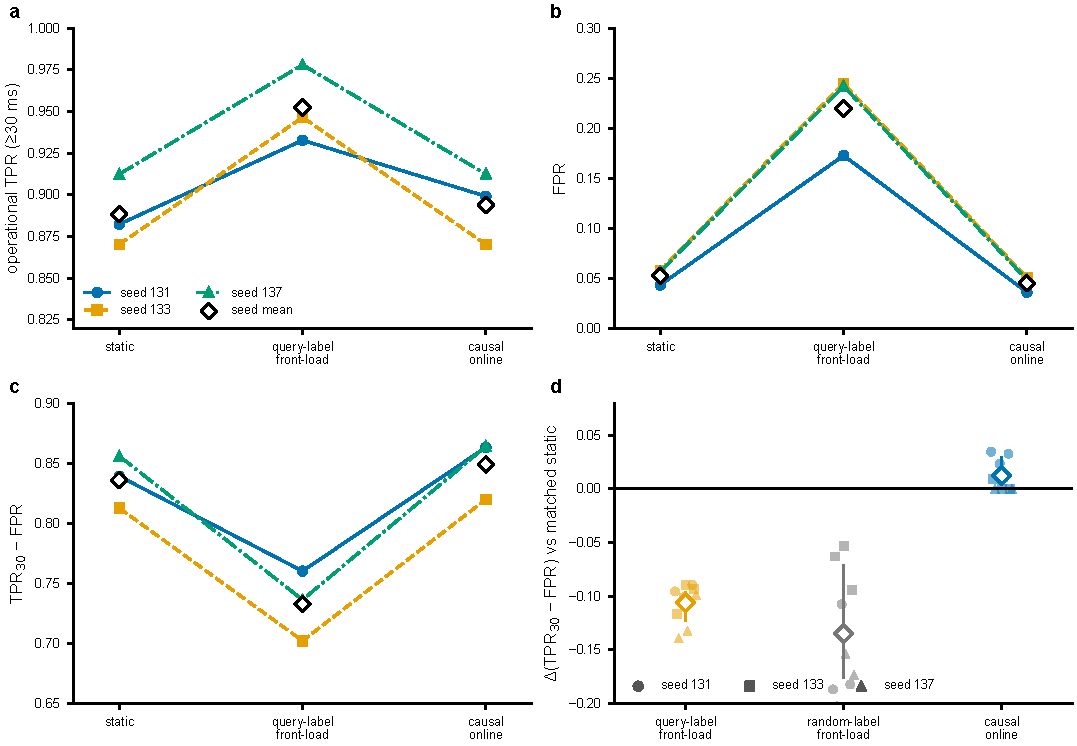
\includegraphics[width=\textwidth]{fig8_equal_label_budget_frontload_ablation.pdf}
  \caption{Same-label-access ablation. (a--c) Each line is one model seed, evaluated on that seed's query-label-disjoint complement; diamonds are equal-seed means. Front-loading the exact queried labels increases lead-qualified sensitivity and warning time but produces a much larger FPR increase, lowering TPR$_{30}$--FPR. (d) Changes from the matched static/support-only parent on common complements. Small points are three block-count-matched random-roster replicates per seed; diamonds are means after averaging replicates within seed. No inferential significance is claimed because balanced360 informed policy development and $n=3$ model seeds.}
  \label{fig:equalbudget}
\end{figure*}

\begin{figure*}[t]
  \centering
  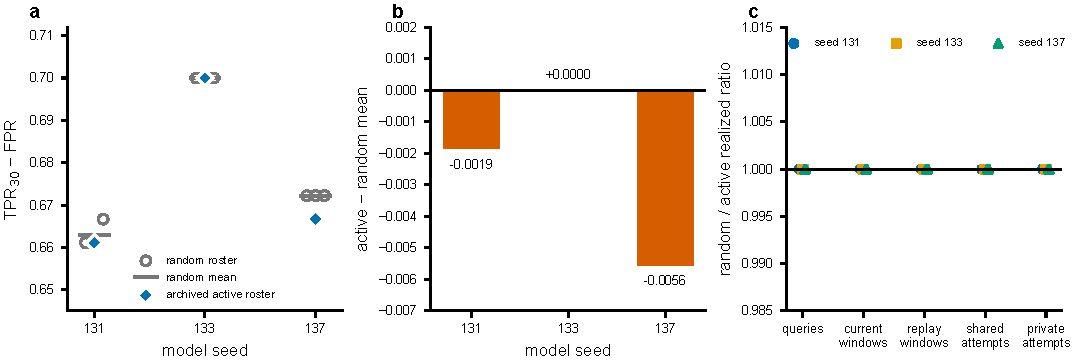
\includegraphics[width=0.88\textwidth]{fig11_equal_compute_selector_screen.pdf}
  \caption{Fixed-shape selector-roster screen on the balanced360 development stream. (a) Archived-active and three block-count-matched random rosters are replayed through the same 16-current/16-support-window, two-shared/two-private-attempt operator. Points are individual random schedules; bars mark their within-seed means. (b) Active-minus-random-mean TPR$_{30}$--FPR does not exceed zero in any seed. (c) Realized window and optimizer-attempt budgets match exactly within seed; guard acceptance and committed parameter changes need not match. This screen rejects archived-roster superiority under this operator; it does not estimate the adaptive policy or prove equivalence or prospective generalization.}
  \label{fig:equalcompute}
\end{figure*}

\begin{figure*}[t]
  \centering
  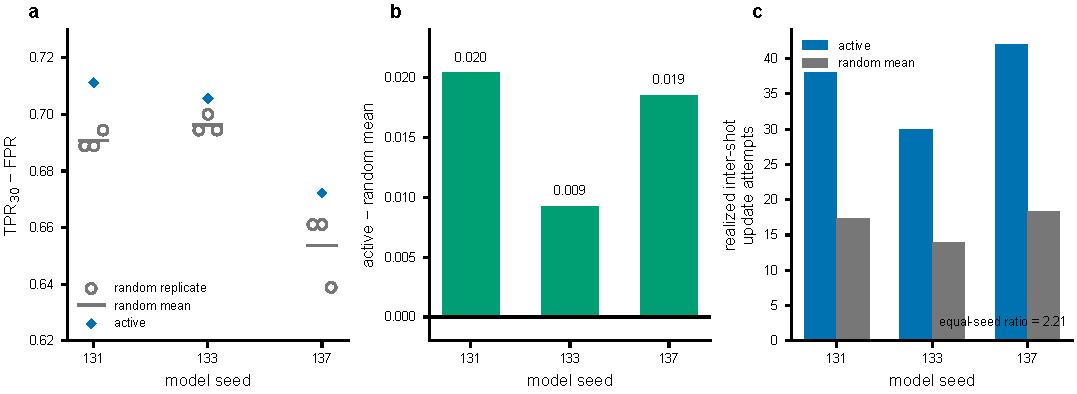
\includegraphics[width=\textwidth]{fig9_active_vs_causal_random_query.pdf}
  \caption{Causal active-versus-random query control on the balanced360 development stream. (a) Diamonds show the active TPR$_{30}$--FPR and open circles show three block-matched random-query replicates for each model seed; horizontal bars are within-seed random means. (b) Active-minus-random-mean differences are positive for all three seeds. (c) Active selection also triggers more realized error-conditioned inter-shot update attempts. Query counts, per-20-shot counts, parents, static predictions, runner and configured step budgets match, but realized compute does not; with three same-direction seeds the exact one-sided sign probability is 0.125.}
  \label{fig:causalrandom}
\end{figure*}

\subsection{Controls, robustness, and an interpretable rescue}

The real episode gate removes eight seed--shot false alarms and loses no operational TP; the full online path also adds four operational TPs relative to static.  In contrast, no-label and one-shot feature-lag screens remove none; one-shot label lag removes one; the archived episode/protected-calibration screens named \texttt{temporal\_zero} and \texttt{raw8\_zero} remove three; label flipping removes two false alarms but loses 23 operational TPs.  The \texttt{raw8\_zero} archive does not preserve a model-level sidecar intervention or a complete trajectory rerun, so it cannot isolate the eight private channels themselves.  Together with the same-label front-load and random-query ablations, these development controls are compatible with, but do not establish, roles for correctly revealed labels, temporal evolution, guarded update timing and target-private observations.  The fixed-operator screen does not support superiority of the archived active roster under that operator; it neither estimates the adaptive selector-policy effect nor proves that query identity made no contribution to the full mechanism.  An independently selected future stream is absent, so the coupled mechanism remains developmental and does not prove recovery of the causal disruption mechanism.

An earlier, separately registered dual-threshold alarm stage tested 37 local/joint parameter perturbations; 31 satisfy operational TPR$\geq0.75$ and FPR$\leq0.20$.  Its registered point is operational TPR 0.800 and FPR 0.122.  A 2,000-repeat bootstrap gives operational TPR $[0.739,0.856]$, so the point estimate does not establish high-confidence sensitivity above 0.8.  This robustness matrix concerns the predecessor alarm stage, not the exact final v3c policy, and is labeled accordingly.

\begin{figure*}[t]
  \centering
  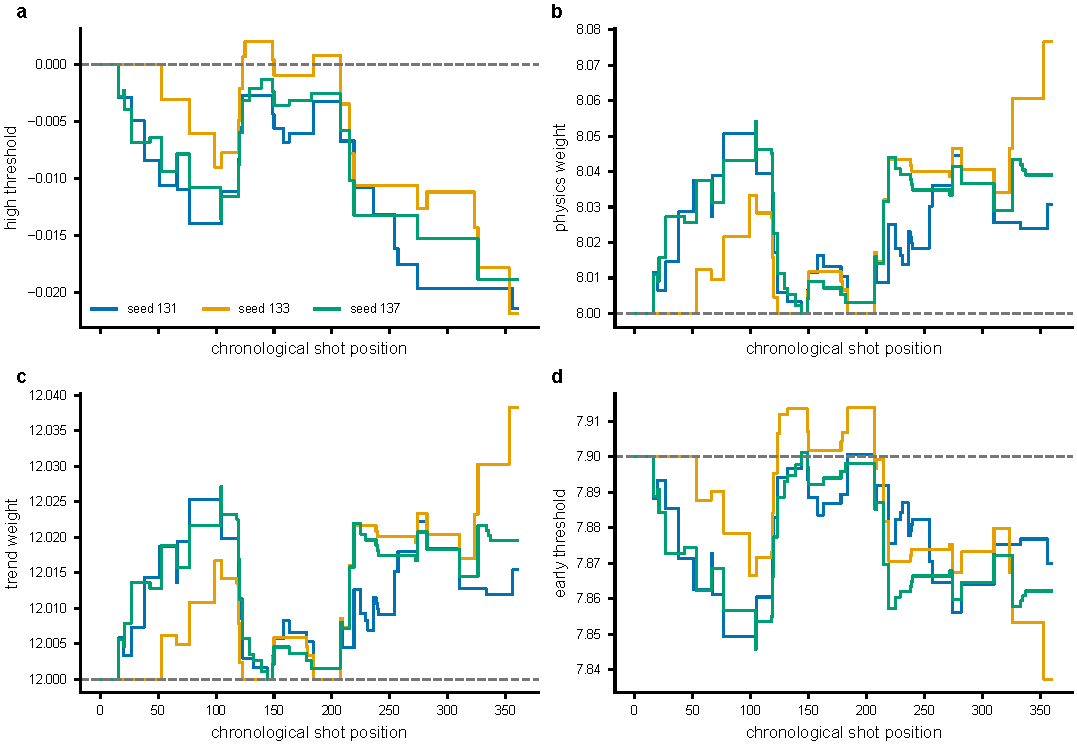
\includegraphics[width=\textwidth]{fig5_adaptive_alarm_state_machine.pdf}
  \caption{Executed multi-parameter alarm adaptation.  Each trajectory is reconstructed from immutable update ledgers in chronological shot order.  Changes occur only after selected label reveal, remain within registered projection bounds, and affect later shots only.}
  \label{fig:alarmstate}
\end{figure*}

Figure~\ref{fig:case} shows safe \east{} shot 73790.  The static model alarms at endpoint 4056 (7.183 s); the online episode model, trained only from previously queried shots, identifies a false-alarm-like temporal segment and blocks it.  Independent physics support can override the block.  This is a useful mechanistic case study, but one selected rescue cannot establish generality.

\begin{figure*}[t]
  \centering
  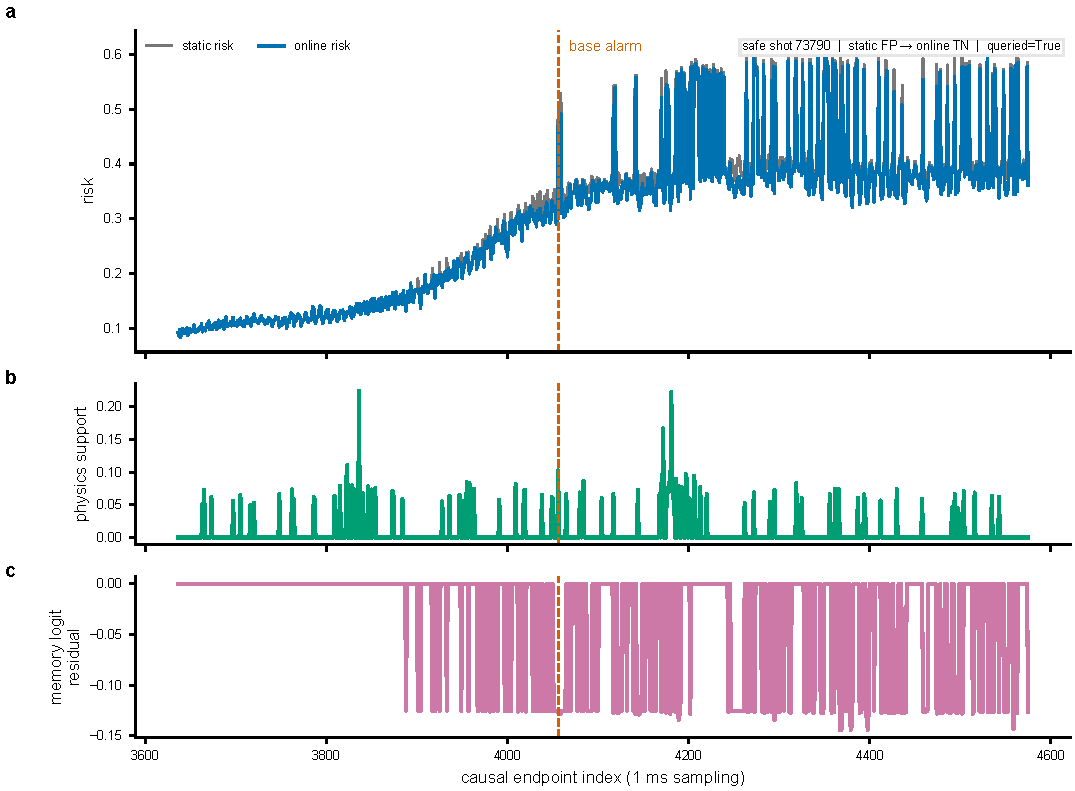
\includegraphics[width=\textwidth]{fig6_causal_false_alarm_rescue_shot73790.pdf}
  \caption{Causal false-alarm rescue for safe shot 73790 (seed 131). The gate uses only the current/past trace and previously queried outcomes, acts after the base supported alarm, and can only delay or veto. The archived episode record gives false-positive probability 0.727, confidence 1.00, and past safe/disruptive support counts 8/23. This selected example is explanatory rather than population-level evidence.}
  \label{fig:case}
\end{figure*}

\begin{figure*}[t]
  \centering
  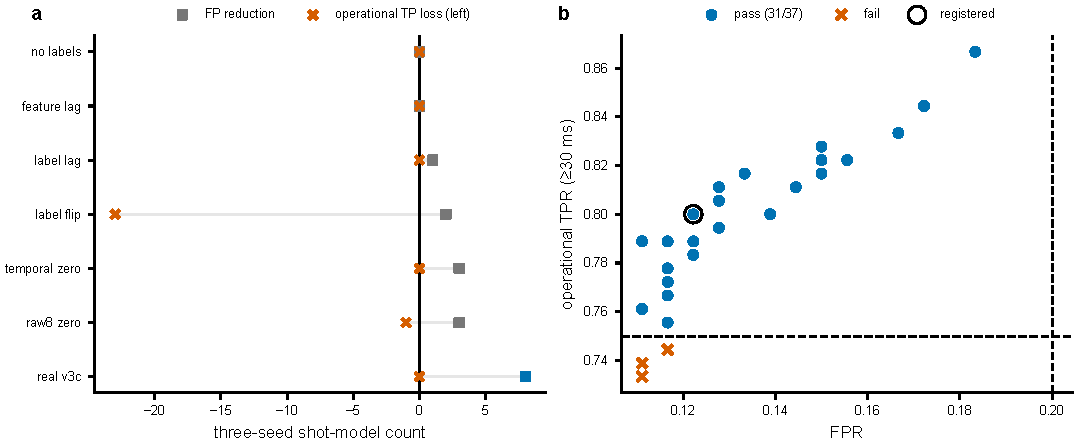
\includegraphics[width=\textwidth]{fig7_negative_controls_and_alarm_robustness.pdf}
  \caption{Negative controls and predecessor alarm robustness. Real v3c has the largest false-alarm reduction without operational-TP loss; 31/37 perturbations pass the predecessor dual-threshold gate. These are development analyses, not multiplicity-corrected confirmation.}
  \label{fig:controls}
\end{figure*}

\clearpage
\section{Discussion}

\paragraph{What changed the transfer outcome.}
The key improvement over failed global alignment was structural, not a small loss-weight change.  First, shared transfer was restricted to 17 features whose semantics can be reconstructed on both devices; target-specific columns were modeled privately.  Second, target dynamics and risk readout were allowed to differ instead of forcing an upper temporal representation to be device invariant, consistent with prior cross-tokamak evidence~\citep{zheng2023transfer}.  Third, outcome labels were spent on errors and protected boundaries under a causal protocol rather than used to retroactively alter current-shot prediction.  Global CORAL/DANN-style alignment remains a historical baseline, not the winning explanation.  Physics-guided domain adaptation can combine adversarial, MMD, reconstruction, and physics losses~\citep{zheng2025phydanet}, but the present evidence does not justify adding those terms when feature support and temporal readout are the dominant mismatch.

\paragraph{Why the result is not ``perfect.''}
Five limitations are decisive.  (i) The primary source representation fails the padding/context gate.  PADFIX demonstrates that this shortcut can be reduced, but the frozen target policy then transfers negatively.  (ii) \jtext{} VAL160/TEST220 are count-aligned, outcome-balanced, non-chronological comparators.  (iii) all support110 shots are reused for target fitting and threshold selection.  (iv) balanced360 informed the method and 972 episode candidates were screened on it; resampling and all label/query controls remain development evidence.  The fixed-shape roster screen closes the realized-window/optimizer-attempt mismatch for its separate assimilation operator, but fails its archived-roster superiority gate and cannot create an unseen test or estimate the adaptive policy.  (v) block-2 FPR and safe-score/shot correlations indicate residual campaign dependence.  In addition, 20--23 disruptive alarms per seed occur more than 3 s before disruption.  They count under the requested metric but are separately flagged because excessive warning can be operationally ambiguous.

\paragraph{Required confirmation.}
Before a deployment or strong external-validity claim, the complete source, support adaptation, alarm formula, query policy, update budget, thresholds, and artifact hashes must be frozen.  One newly acquired chronological \east{} stream must then be predicted without model selection, with outcomes released only according to the registered online budget.  The confirmation should require all three seeds to satisfy overall and worst-block gates, test early-alarm distributions and shot/campaign correlations, and compare static, active, random-query, no-label, and feature/time-shift controls at equal compute.  Until then, the correct status is \devstatus{}.

\section{Conclusion}

The study establishes a fully executable \jtext{} source $\rightarrow$ \east{} few-shot transfer $\rightarrow$ \east{} online-active chain and gives its three same-lineage development metrics, causal ledgers, and failure audits.  On the reused development stream, the selected policy records a mean FPR change from 0.167 to 0.152 and operational TPR change from 0.841 to 0.848, corresponding to eight fewer seed--shot false alarms and four additional lead-qualified TPs.  Front-loading the same queried labels increases sensitivity but degrades TPR$_{30}$--FPR in all seeds, showing that target-label count alone is insufficient to reproduce the online operating point.  Conversely, the fixed-shape roster screen finds no archived-roster superiority under its new operator, so the original online result remains a coupled effect of label timing, error-triggered assimilation, replay, rollback and alarm protection.  The stronger scientific contribution is this falsifiable boundary: nominally matching channel indices are not automatically transferable; development controls are compatible with roles for target-private observations and temporal dynamics; causal label use is executable; and both source-shortcut repair and roster isolation can overturn a favorable aggregate narrative.  Independent future-stream confirmation remains required.

\section*{Data availability}

The reproducibility package records exact shot rosters, roster SHA-256 values, HDF5 field contracts, and machine-readable derived evidence.  Raw HDF5 data are external and no public DOI or controlled-access route has yet been established in this development copy.  Consequently, third-party end-to-end reproduction remains blocked until the authors deposit the data or publish an access procedure; outcome labels are never reconstructed from prose tables.

\section*{Code availability}

The local package contains metric builders, frozen command plans, per-shot ledgers, tests, figure source data and hashes, and compiled supplementary material.  It has not yet been archived in a public versioned repository with a DOI.  The release candidate therefore supports local audit but does not yet satisfy the archival code-availability condition for submission.

\section*{Computational resources}

The recorded runs used a single NVIDIA GeForce RTX 5070 Laptop GPU (8,151 MiB) in the \texttt{rl\_env} CUDA environment.  Source-training wall times were 46.8, 73.1, and 58.8 s for seeds 131/133/137.  Update counts and model-state hashes are archived, but target/online wall time, FLOPs, and energy were not captured by the historical runner and must not be inferred retroactively.

\section*{AI-assisted development disclosure}

Generative-AI assistance was used for code review, evidence-pipeline edits, figure/manuscript drafting, and language editing.  It is not an author.  Named authors must verify every claim, contribution, citation, and artifact before submission.

\section*{Author contributions and competing interests}

Author names, contribution taxonomy, acknowledgements, funding, and competing-interest declarations are intentionally not fabricated in this anonymous development copy and must be completed by the authors before submission.

\section*{Ethics and operational safety}

No result in this development study should directly trigger plasma-control actions.  Deployment requires device-operator review, latency and missing-channel validation, fail-safe integration, and prospective confirmation under a predeclared operating policy.

\bibliographystyle{unsrtnat}
\bibliography{references}

\end{document}
